%%%%%%%%%%%%%%%%%%%%%%%%%%%%%%%%%%%%%%%%%
% Programming/Coding Assignment
% LaTeX Template
%
% This template has been downloaded from:
% http://www.latextemplates.com
%
% Original author:
% Ted Pavlic (http://www.tedpavlic.com)
%
% Note:
% The \lipsum[#] commands throughout this template generate dummy text
% to fill the template out. These commands should all be removed when 
% writing assignment content.
%
% This template uses a Perl script as an example snippet of code, most other
% languages are also usable. Configure them in the "CODE INCLUSION 
% CONFIGURATION" section.
%
%%%%%%%%%%%%%%%%%%%%%%%%%%%%%%%%%%%%%%%%%

%----------------------------------------------------------------------------------------
%	PACKAGES AND OTHER DOCUMENT CONFIGURATIONS
%----------------------------------------------------------------------------------------

\documentclass{article}

\usepackage{fancyhdr} % Required for custom headers
\usepackage{lastpage} % Required to determine the last page for the footer
\usepackage{extramarks} % Required for headers and footers
\usepackage[usenames,dvipsnames]{color} % Required for custom colors
\usepackage{graphicx} % Required to insert images
\usepackage{listings} % Required for insertion of code
\usepackage{courier} % Required for the courier font
\usepackage{lipsum} % Used for inserting dummy 'Lorem ipsum' text into the template
\usepackage{setspace}
\usepackage{color}
\usepackage{comment}
\usepackage{caption}

\usepackage{hyperref}
\usepackage{natbib}
\usepackage{underscore}
\usepackage{subfigure}
\usepackage{fixltx2e}

\hypersetup{
    colorlinks=true,
    linkcolor=blue,
    filecolor=magenta,      
    urlcolor=cyan,
    breaklinks=true
}

%\usepackage[]{algorithm2e}
\usepackage{pdfpages}




%For python inclusion (http://widerin.org/blog/syntax-highlighting-for-python-scripts-in-latex-documents)
\definecolor{Code}{rgb}{0,0,0}
\definecolor{Decorators}{rgb}{0.5,0.5,0.5}
\definecolor{Numbers}{rgb}{0.5,0,0}
\definecolor{MatchingBrackets}{rgb}{0.25,0.5,0.5}
\definecolor{Keywords}{rgb}{0,0,1}
\definecolor{self}{rgb}{0,0,0}
\definecolor{Strings}{rgb}{0,0.63,0}
\definecolor{Comments}{rgb}{0,0.63,1}
\definecolor{Backquotes}{rgb}{0,0,0}
\definecolor{Classname}{rgb}{0,0,0}
\definecolor{FunctionName}{rgb}{0,0,0}
\definecolor{Operators}{rgb}{0,0,0}
\definecolor{Background}{rgb}{0.98,0.98,0.98}

\newcommand*{\srcPath}{../src}%

\lstset{
	basicstyle=\footnotesize,
	breaklines=true,
}

% Margins
\topmargin=-0.45in
\evensidemargin=0in
\oddsidemargin=0in
\textwidth=6.5in
\textheight=9.0in
\headsep=0.25in

\linespread{1.1} % Line spacing

% Set up the header and footer
\pagestyle{fancy}
\lhead{\hmwkAuthorName} % Top left header
%\chead{\hmwkClass\ (\hmwkClassInstructor\ \hmwkClassTime): \hmwkTitle} % Top center head
\chead{\hmwkClass\ (\hmwkClassInstructor): \hmwkTitle} % Top center head
\rhead{\firstxmark} % Top right header
\lfoot{\lastxmark} % Bottom left footer
\cfoot{} % Bottom center footer
\rfoot{Page\ \thepage\ of\ \protect\pageref{LastPage}} % Bottom right footer
\renewcommand\headrulewidth{0.4pt} % Size of the header rule
\renewcommand\footrulewidth{0.4pt} % Size of the footer rule

\setlength\parindent{0pt} % Removes all indentation from paragraphs

%----------------------------------------------------------------------------------------
%	CODE INCLUSION CONFIGURATION
%----------------------------------------------------------------------------------------

\definecolor{MyDarkGreen}{rgb}{0.0,0.4,0.0} % This is the color used for comments
\lstloadlanguages{Perl} % Load Perl syntax for listings, for a list of other languages supported see: ftp://ftp.tex.ac.uk/tex-archive/macros/latex/contrib/listings/listings.pdf
\lstset{language=Perl, % Use Perl in this example
        frame=single, % Single frame around code
        basicstyle=\small\ttfamily, % Use small true type font
        keywordstyle=[1]\color{Blue}\bf, % Perl functions bold and blue
        keywordstyle=[2]\color{Purple}, % Perl function arguments purple
        keywordstyle=[3]\color{Blue}\underbar, % Custom functions underlined and blue
        identifierstyle=, % Nothing special about identifiers                                         
        commentstyle=\usefont{T1}{pcr}{m}{sl}\color{MyDarkGreen}\small, % Comments small dark green courier font
        stringstyle=\color{Purple}, % Strings are purple
        showstringspaces=false, % Don't put marks in string spaces
        tabsize=5, % 5 spaces per tab
        %
        % Put standard Perl functions not included in the default language here
        morekeywords={rand},
        %
        % Put Perl function parameters here
        morekeywords=[2]{on, off, interp},
        %
        % Put user defined functions here
        morekeywords=[3]{test},
       	%
        morecomment=[l][\color{Blue}]{...}, % Line continuation (...) like blue comment
        numbers=left, % Line numbers on left
        firstnumber=1, % Line numbers start with line 1
        numberstyle=\tiny\color{Blue}, % Line numbers are blue and small
        stepnumber=5 % Line numbers go in steps of 5
}

% Creates a new command to include a perl script, the first parameter is the filename of the script (without .pl), the second parameter is the caption
\newcommand{\perlscript}[2]{
\begin{itemize}
\item[]\lstinputlisting[caption=#2,label=#1]{#1.pl}
\end{itemize}
}


%----------------------------------------------------------------------------------------
%	DOCUMENT STRUCTURE COMMANDS
%	Skip this unless you know what you're doing
%----------------------------------------------------------------------------------------

% Header and footer for when a page split occurs within a problem environment
\newcommand{\enterProblemHeader}[1]{
\nobreak\extramarks{#1}{#1 continued on next page\ldots}\nobreak
\nobreak\extramarks{#1 (continued)}{#1 continued on next page\ldots}\nobreak
}

% Header and footer for when a page split occurs between problem environments
\newcommand{\exitProblemHeader}[1]{
\nobreak\extramarks{#1 (continued)}{#1 continued on next page\ldots}\nobreak
\nobreak\extramarks{#1}{}\nobreak
}

\setcounter{secnumdepth}{0} % Removes default section numbers
\newcounter{homeworkProblemCounter} % Creates a counter to keep track of the number of problems

\newcommand{\homeworkProblemName}{}
\newenvironment{homeworkProblem}[1][Problem \arabic{homeworkProblemCounter}]{ % Makes a new environment called homeworkProblem which takes 1 argument (custom name) but the default is "Problem #"
\stepcounter{homeworkProblemCounter} % Increase counter for number of problems
\renewcommand{\homeworkProblemName}{#1} % Assign \homeworkProblemName the name of the problem
\section{\homeworkProblemName} % Make a section in the document with the custom problem count
\enterProblemHeader{\homeworkProblemName} % Header and footer within the environment
}{
\exitProblemHeader{\homeworkProblemName} % Header and footer after the environment
}

\newcommand{\problemAnswer}[1]{ % Defines the problem answer command with the content as the only argument
\noindent\framebox[\columnwidth][c]{\begin{minipage}{0.98\columnwidth}#1\end{minipage}} % Makes the box around the problem answer and puts the content inside
}

\newcommand{\homeworkSectionName}{}
\newenvironment{homeworkSection}[1]{ % New environment for sections within homework problems, takes 1 argument - the name of the section
\renewcommand{\homeworkSectionName}{#1} % Assign \homeworkSectionName to the name of the section from the environment argument
\subsection{\homeworkSectionName} % Make a subsection with the custom name of the subsection
\enterProblemHeader{\homeworkProblemName\ [\homeworkSectionName]} % Header and footer within the environment
}{
\enterProblemHeader{\homeworkProblemName} % Header and footer after the environment
}

%----------------------------------------------------------------------------------------
%	NAME AND CLASS SECTION
%----------------------------------------------------------------------------------------
%#MOD
\newcommand{\hmwkTitle}{Assignment\ \#6 } % Assignment title
%\newcommand{\hmwkDueDate}{Monday,\ January\ 1,\ 2012} % Due date
\newcommand{\hmwkClass}{Web Science} % Course/class
%\newcommand{\hmwkClassTime}{10:30am} % Class/lecture time
\newcommand{\hmwkClassInstructor}{Alexander Nwala} % Teacher/lecturer
\newcommand{\hmwkAuthorName}{Mohd. Nauman Siddique} % Your name

%----------------------------------------------------------------------------------------
%	TITLE PAGE
%----------------------------------------------------------------------------------------

\title{
\vspace{2in}
\textmd{\textbf{\hmwkClass:\ \hmwkTitle}}\\
%\normalsize\vspace{0.1in}\small{Due\ on\ \hmwkDueDate}\\
%\vspace{0.1in}\large{\textit{\hmwkClassInstructor\ \hmwkClassTime}}
\vspace{0.1in}\large{\textit{\hmwkClassInstructor}}
\vspace{3in}
}

\author{\textbf{\hmwkAuthorName}}
%#MOD
\date{Sunday, March 31, 2019} % Insert date here if you want it to appear below your name

%----------------------------------------------------------------------------------------

\begin{document}

\maketitle



%----------------------------------------------------------------------------------------
%	TABLE OF CONTENTS
%----------------------------------------------------------------------------------------

%\setcounter{tocdepth}{1} % Uncomment this line if you don't want subsections listed in the ToC

\newpage
\tableofcontents
\newpage

%----------------------------------------------------------------------------------------
%	PROBLEM 1
%----------------------------------------------------------------------------------------

% To have just one problem per page, simply put a \clearpage after each problem

\begin{homeworkProblem}


Create a blog-term matrix.  Start by grabbing 100 blogs hosted on https://www.blogger.com. Include:

http://f-measure.blogspot.com/
http://ws-dl.blogspot.com/

The method described in class no longer works. So use your discretion to 
grab 98 more blogs. Describe how you generated the blog data - manually or
automatically. Note that each student will separately do
this process, so it is unlikely that these 98 blogs will be shared
among students.  In other words, no sharing of blog data.  Upload
to github your code (if you used one) for grabbing the blogs and provide a list of
blog URIs, both in the report and in github.

Use the blog title as the identifier for each blog (and row of the
matrix).  Use the terms from every item/title (RSS) or entry/title
(Atom) for the columns of the matrix.  The values are the frequency
of occurrence.  Essentially you are replicating the format of the
"blogdata.txt" file included with the PCI book code.  Limit the
number of terms to the most "popular" (i.e., frequent) 1000 terms,
this is *after* the criteria on p. 32 (chapter 3 PCI book) (slide 8 - Week 11) has been satisfied. Remember that blogs are paginated (slide 46).  

%\problemAnswer
%{
    \begin{verbatim}\end{verbatim}
    \textbf{SOLUTION}\\

To solve this problem I decided to write a shell script called \textbf{grabBlogs.py} to retrieve the 98 random blogs as shown in Listing \ref{lst:grabBlogs}. The script utilizes mainly utilizes the blogger url for profile search using a query parameter to solve the problem of retrieving unique blogs. The blogger url \url{http://www.blogger.com/profile-find.g?t=m&q=} called each time with search query parameter to retrieve 200 blogs. I used 200 executions because I happened to get duplicate blogs on some occasions and 100 calls wouldn't be enough to satisfy the requirements of this problem. For each new blog I got I saved the contents of the html page to a html document with the an id of the current iteration in the range of 200. I saved this file id and the URI found inside a file called \textbf{blogList.txt} as shown in Listing \ref{lst:blogList}.

After 200 blogs were retrieved I used the sort command to find all unique blogs in the blog list file. Once this completed I had approximately 120 unique blogs. I then wrote a script in python 3.6 called \textbf{getFeed.py} as shown in Listing \ref{lst:getFeed} which parsed each html document saved using the library Beautiful soup which allowed me to search the document by an HTML `link` element to find the atom+xml feed of the blog. I saved these feeds to a file called \textbf{feedList.txt} which was later cleaned for any blogs that did not have atom+xml feeds. Usually these were blogs that no longer existed. Any extra blogs above 100 were simply discarded.

Finally I proceeded to to write another python script called \textbf{generateFeedVector.py} shown in Listing \ref{lst:generateMat} which utilized the code provide by the Programming Collective Intelligence (PCI) book. This script was slightly modified to be usable for python 3.6 but also adding a limit to the amount of words the blog-term matrix allowed to a maximum of 1000 shown on line 65. I also didn't check for stop words when I retrieved the atom feeds, but I did check if words were stop words before creating the the matrix by using the nltk library's corpus of stop words shown on line 28. If a word was found to be a stop word according to their corpus it would not be added to the matrix. When this was completed it was saved to a file called \textbf{blogData.txt}.

 \lstinputlisting[frame=single,caption={Pythonl script to retrieve unique blogs},label=lst:grabBlogs,captionpos=b,numbers=left,showspaces=false,showstringspaces=false,basicstyle=\footnotesize]{\srcPath/grabBlogs.py}

 \lstinputlisting[frame=single,caption={100 unique blogs collected},label=lst:blogList,captionpos=b,numbers=left,showspaces=false,showstringspaces=false,basicstyle=\footnotesize]{\srcPath/data/BlogUrls.txt}

 \lstinputlisting[frame=single,caption={Python script to retrieve atom feeds of blogs},label=lst:getFeed,captionpos=b,numbers=left,showspaces=false,showstringspaces=false,basicstyle=\footnotesize]{\srcPath/getFeed.py}

 \lstinputlisting[frame=single,caption={Python script to generate blog-term matrix},label=lst:generateMat,captionpos=b,numbers=left,showspaces=false,showstringspaces=false,basicstyle=\footnotesize]{\srcPath/generateFeedVector.py}
  
%}

\end{homeworkProblem}

%----------------------------------------------------------------------------------------
%   PROBLEM 2
%----------------------------------------------------------------------------------------

\begin{homeworkProblem}

Create an ASCII and JPEG dendrogram that clusters (i.e., HAC)
the most similar blogs (see slides 13 \& 14).  Include the JPEG in
your report and upload the ascii file to github (it will be too
unwieldy for inclusion in the report).
%\problemAnswer
%{
    \begin{verbatim}\end{verbatim}
    \textbf{SOLUTION}\\
To solve this question I used the code provided by the Programming Collective Intelligence book to write a script in python 2.7 called \textbf{createClusters.py} as shown in Listing \ref{lst:createClusters}. This script has a method called \textit{createDendrogram} which utilizes the clusters.py file provided by the PCI book load the blog-term matrix created in question 1 to create a Hierarchical Clustering tree image, the dendrogram, as shown in Figure \ref{fig:dendro}. I also created an ASCII file named \textbf{q2ASCII.txt} to represent this tree structure in text which is available on my Github page.

 \begin{figure}[h]
 \centering
 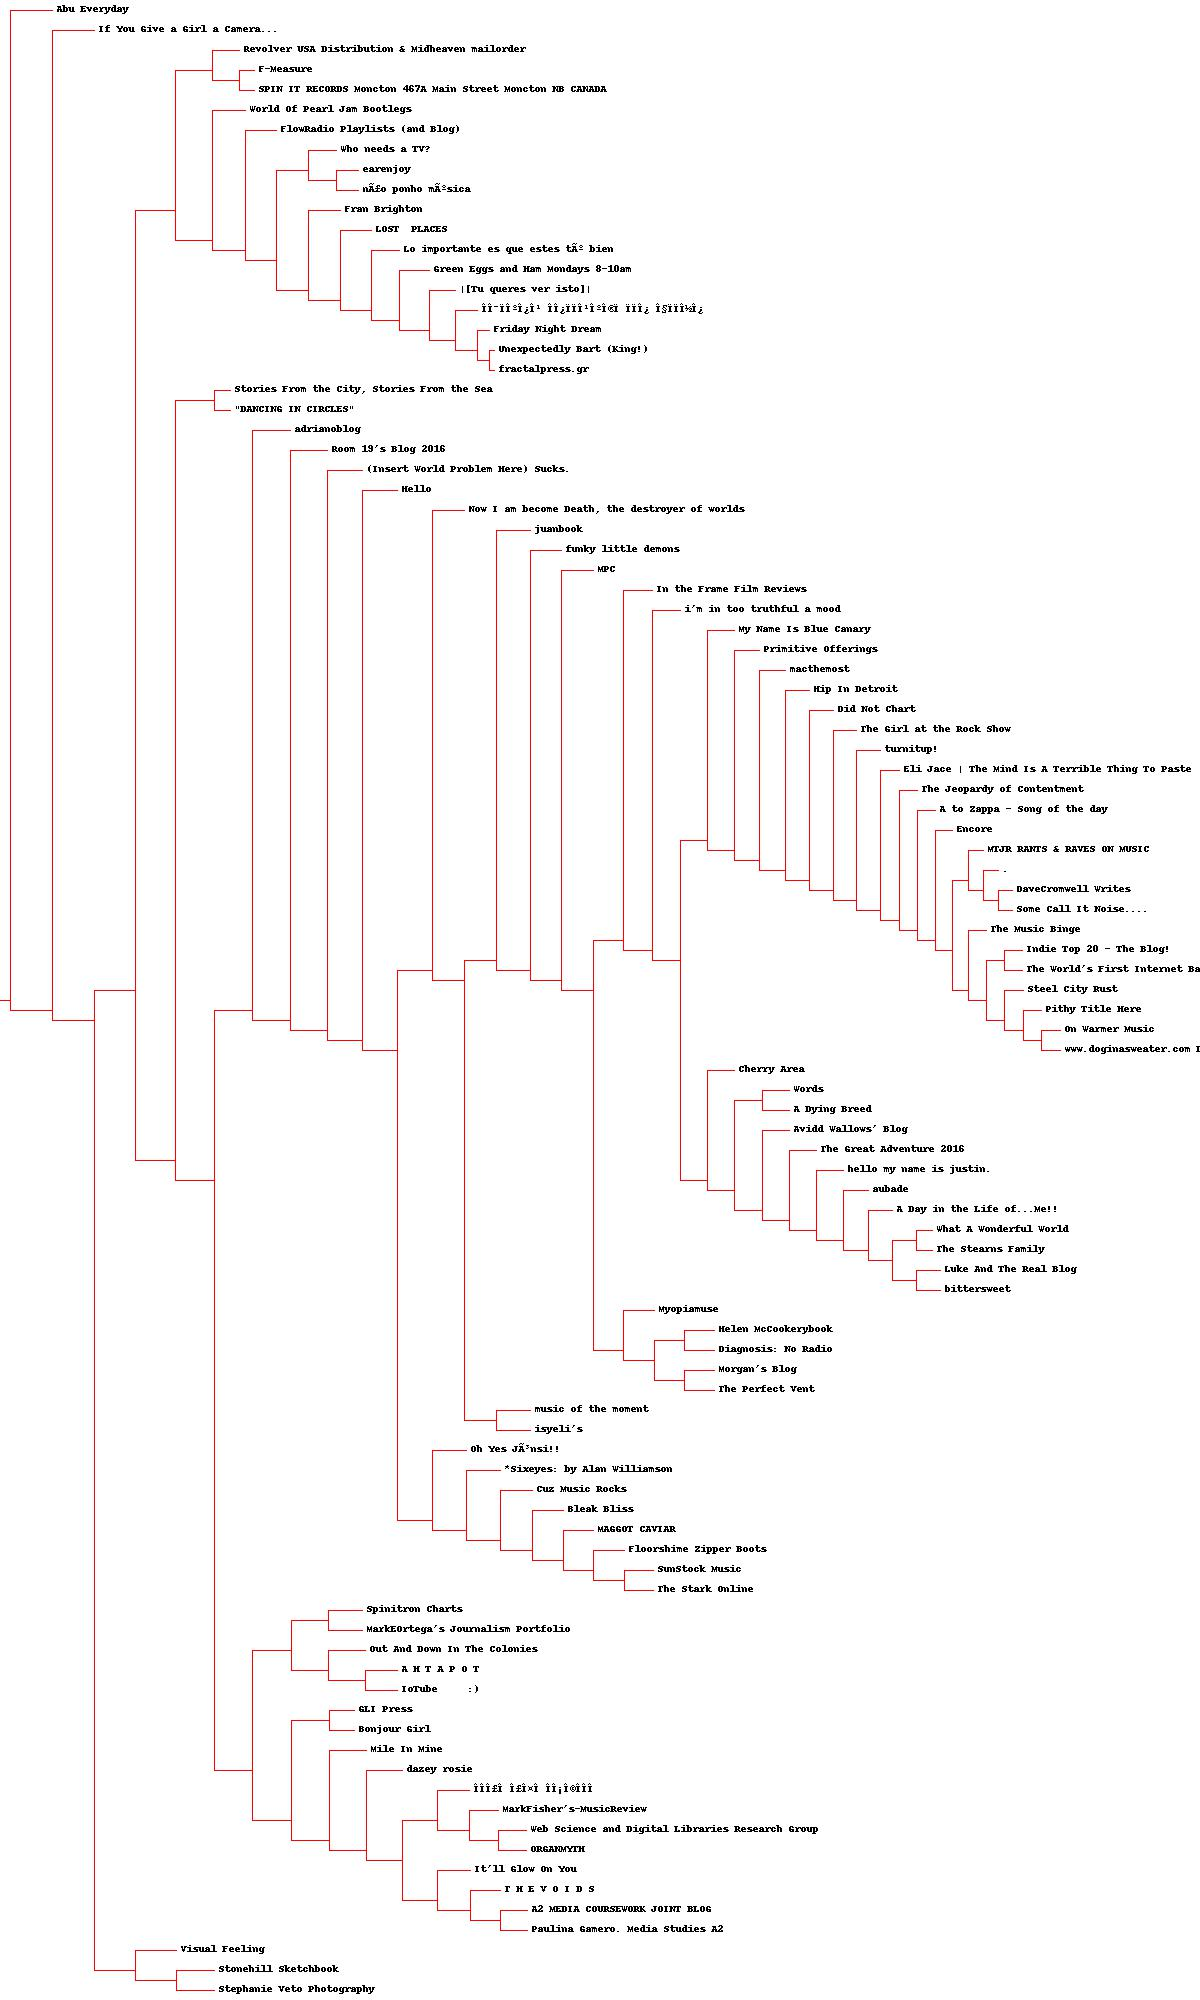
\includegraphics[scale=0.26]{dendogram.png}
 \caption{Dendrogram for blogs collected}
 \label{fig:dendro}
 \end{figure}

\clearpage

 \lstinputlisting[frame=single,caption={Python script to generate clusters with different approaches},label=lst:createClusters,captionpos=b,numbers=left,showspaces=false,showstringspaces=false,basicstyle=\footnotesize]{\srcPath/createClusters.py}

\clearpage
%}

\end{homeworkProblem}

%----------------------------------------------------------------------------------------
%   PROBLEM 3
%----------------------------------------------------------------------------------------

\begin{homeworkProblem}


Cluster the blogs using K-Means, using k=5,10,20. (see slide 
25).  Print the values in each centroid, for each value of k.  How
many iterations were required for each value of k?
%\problemAnswer
%{
    \begin{verbatim}\end{verbatim}
    \textbf{SOLUTION}\\
To solve this question I again used the code provided by the Programming Collective Intelligence book as shown in Listing \ref{lst:createClusters} to create a method called \textit{kmeans}. The \textit{kmeans} method again reads my blog-term matrix and using the method \textit{kcluster} for the clusters.py library. I modified the \textit{kcluster} method to also return the iteration count so it could be saved along with the blog title. For each value of k I created a separate file named \textbf{kclut\_n.txt} where n is the value of k. For a k value of 5 it took 7 iterations with the values of each centroids shown in Listing \ref{lst:kclust5}. For a k value of 10 it took 5 iterations with the values of each centroids shown in Listing \ref{lst:kclust10}. For a k value of 20 it took 5 iterations with the values of each centroids shown in Listing \ref{lst:kclust20}.

 \lstinputlisting[frame=single,caption={K-means clustering with a value of 5},label=lst:kclust5,captionpos=b,numbers=left,showspaces=false,showstringspaces=false,basicstyle=\footnotesize]{\srcPath/data/kclust5.txt}

 \lstinputlisting[frame=single,caption={K-means clustering with a value of 10},label=lst:kclust10,captionpos=b,numbers=left,showspaces=false,showstringspaces=false,basicstyle=\footnotesize]{\srcPath/data/kclust10.txt}

 \lstinputlisting[frame=single,caption={K-means clustering with a value of 20},label=lst:kclust20,captionpos=b,numbers=left,showspaces=false,showstringspaces=false,basicstyle=\footnotesize]{\srcPath/data/kclust20.txt}


%}

\end{homeworkProblem}

%----------------------------------------------------------------------------------------
%   PROBLEM 4
%----------------------------------------------------------------------------------------

\begin{homeworkProblem}

Use MDS to create a JPEG of the blogs similar to slide 29 of the 
week 11 lecture.  How many iterations were required?
%\problemAnswer
%{
    \begin{verbatim}\end{verbatim}
    \textbf{SOLUTION}\\
To solve this question I again used the code provided by the Programming Collective Intelligence book as shown in Listing \ref{lst:createClusters} to create a method called \textit{mds}. The \textit{mds} method again reads my blog-term matrix and this time uses the method \textit{scaledown} in the clusters.py library. I modified the \textit{scaledown} method to also return the iteration count so it could be saved along with the blog title. The \textit{mds} method then utilizes the data it takes from my blog-term matrix and utilizes multidimensional scaling (MDS) to create a visual representation of the distance matrix in two dimensions created from the \textit{scaledown} method. The MDS visualization is shown in Figure \ref{fig:mds}. The iteration count was 209 as shown in Figure \ref{fig:scaledown}.

 \begin{figure}[h]
 \centering
 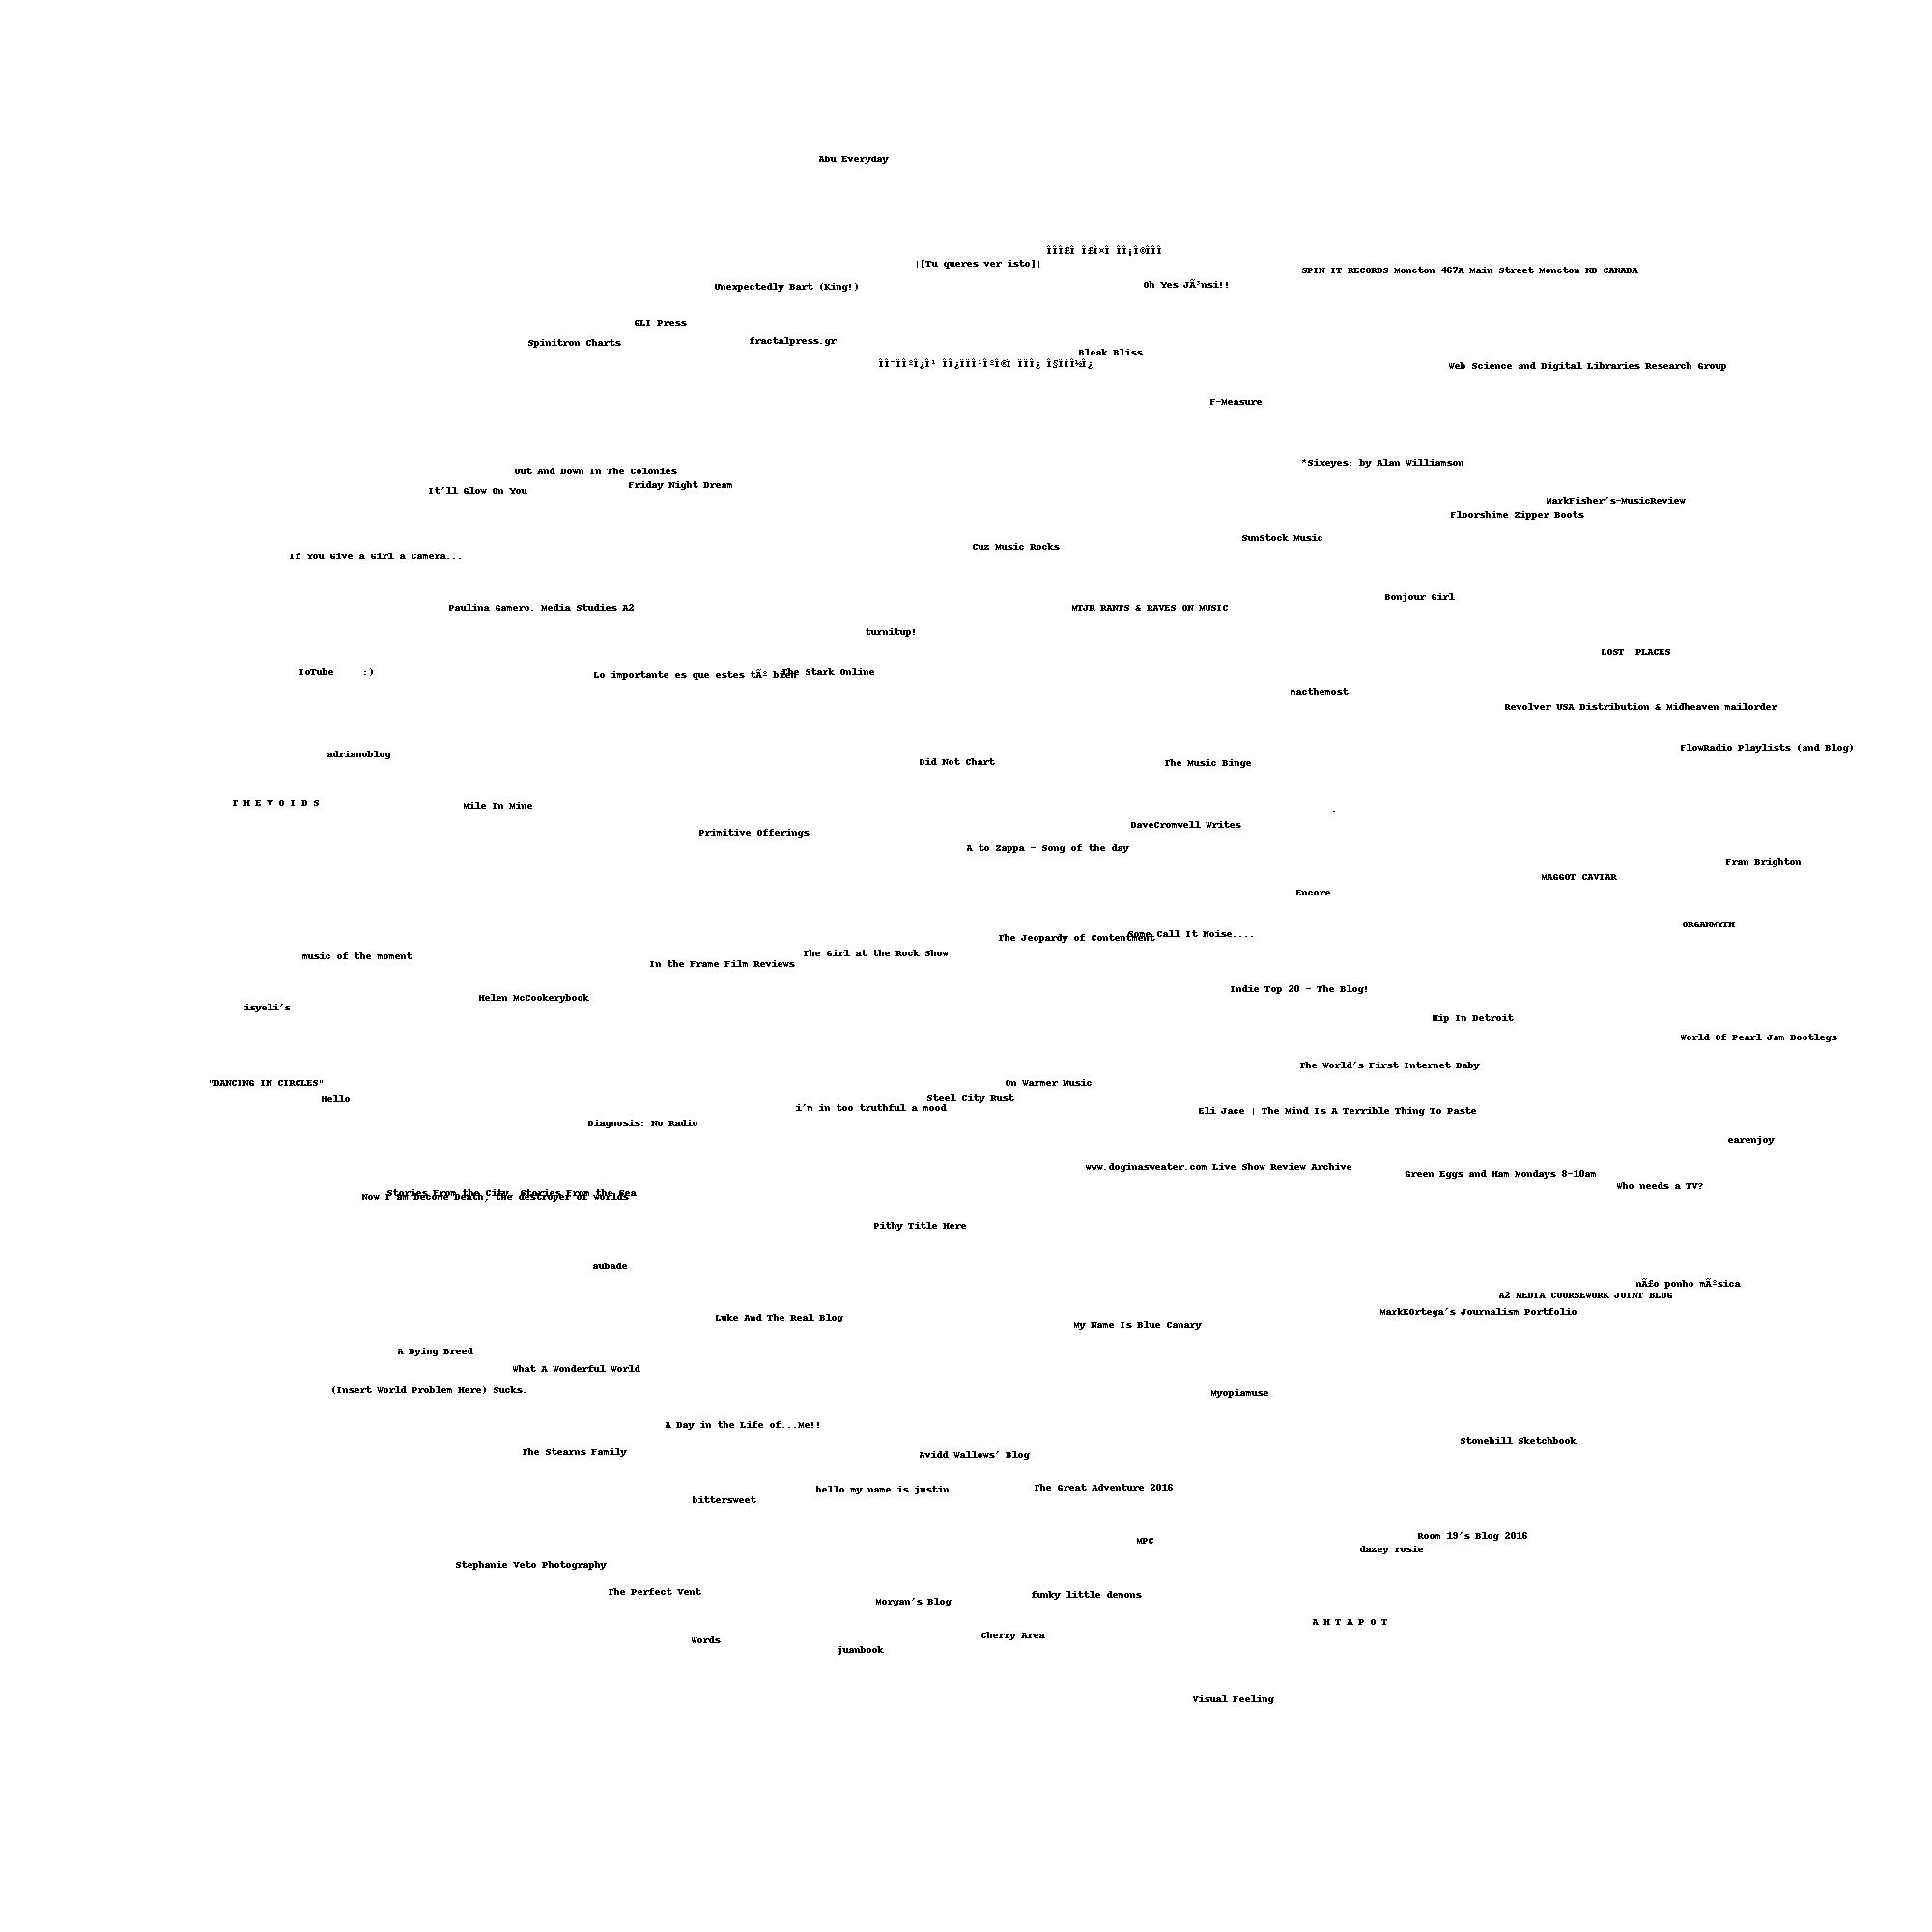
\includegraphics[scale=0.2]{mds.png}
 \caption{Two dimensional representation of blogs}
 \label{fig:mds}
 \end{figure}

 \begin{figure}[h]
 \centering
 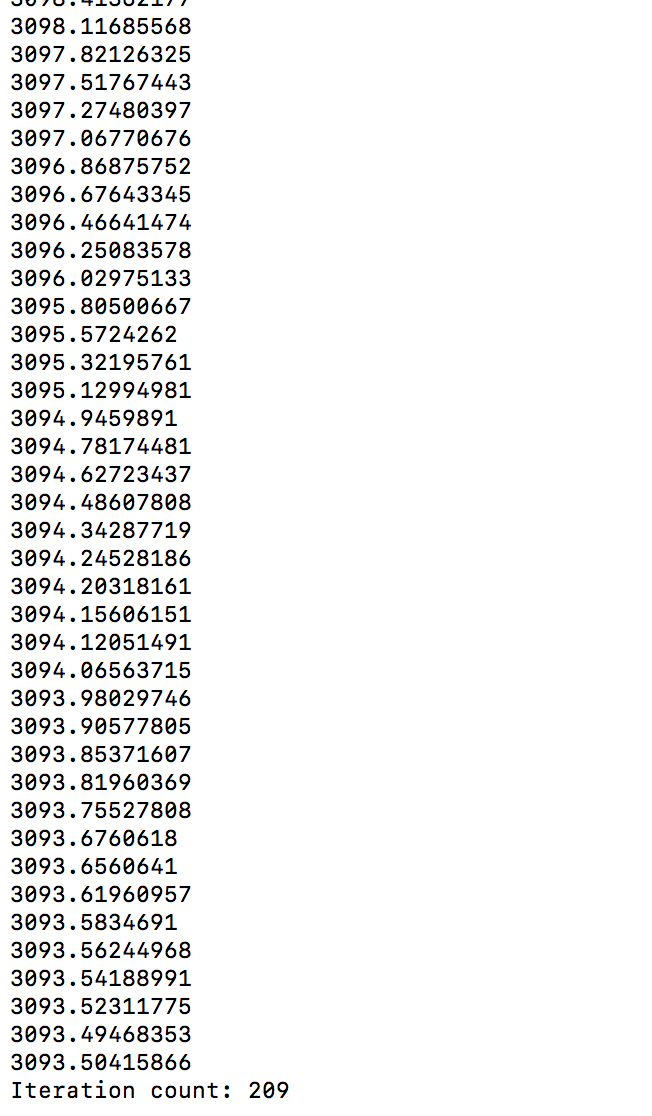
\includegraphics[scale=0.75]{q4itercount}
 \caption{Command line view of the iteration count for MDS}
 \label{fig:scaledown}
 \end{figure}


%}

\end{homeworkProblem}

\end{document}
    


   

    

    

    
   
